\section{Methodological preliminaries}
\label{sec:prelims}

Our first set of experiments, \exptrefrange{exp:prelims-dv}{exp:prelims-frame}, establish the simple reference games in Figure \ref{fig:ex} as a viable method, testing the replicability of judgments in this paradigm and examining particular experimental decisions. 

\begin{figure}[t]
  \centering
  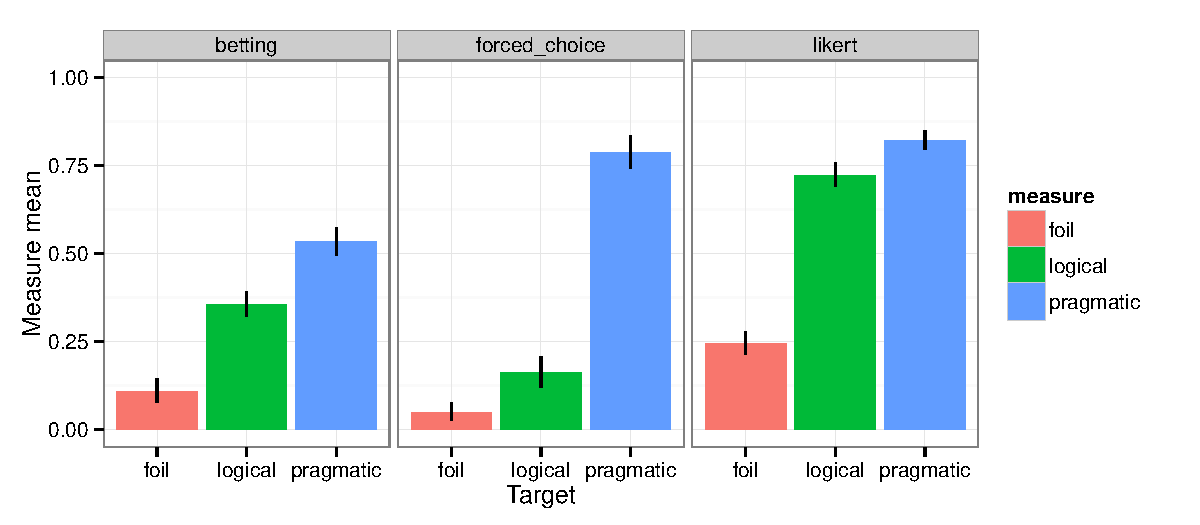
\includegraphics[width=6in]{../plots/1-prelims-dv.pdf}
  \caption{\label{fig:prelims-dv} Data from \exptref{exp:prelims-dv}. Each panel shows results from a different dependent variable (normalized for simplicity into the interval [0,1]. The three columns show results for the foil (e.g., face with nothing), logical (e.g., face with hat and glasses), and pragmatic (face with only glasses) targets. Error bars show 95\% confidence intervals, computed by non-parametric bootstrap.}
\end{figure}

Experiment \exptref{exp:prelims-dv} explored the use of different dependent variables. We considered a betting measure, in which participants were instructed to allocate \$100 across the three targets, as in \citeA{frank2012}; a 7-point Likert scale, as in \citeA{goodman2013}; and a simple three-alternative forced choice measure.\footnote{As this experiment was one of our first, we used only four of our six stimulus items: faces, boats, snowmen, and sundaes.} Figure \ref{fig:prelims-dv} shows results from each. With all three dependent variables, the pragmatic target was chosen more than the logical target, but this result was strongest for the forced choice, with 79\% of participants choosing the pragmatic target. Both the Likert and betting measures afforded the possibility of ``hedging'' by allocating equal bets or ratings to the pragmatic and logical targets. Conservative participants took advantage of this possibility very frequently, betting equal amounts on the logical and pragmatic targets 43\% of the time and using equal Likert ratings 46\% of the time. In contrast, the forced-choice did not allow this kind of hedging; thus, we adopt it in our further experiments.  

Experiment \exptref{exp:prelims-mc} was designed to ensure that the presence of the manipulation check--asking participants to count how many of each feature was present---did not induce a task demand that changed the magnitude of pragmatic responding. We saw 83\% pragmatic responding in the manipulation check condition and 77\% pragmatic responding in a matched condition with no manipulation check. Because of the high power of this experiment ($N_{include}$ = 513), the difference between conditions was statistically significant ($\chi^2(2) = 6.97,~p = .03$). Nevertheless, the modest (6\%) difference between conditions suggests that the manipulation check does not \emph{create} the pragmatic effect, though it may heighten participants' attentions to the different distributions of the two features, leading to slightly more pragmatic responding. We continue to use the manipulation check as an exclusion criterion in further experiments. 

Experiment \exptref{exp:prelims-frame} was designed to test the particular linguistic framing we used, in particular contrasting the presentation of the target word (e.g. ``glasses'') as part of a phrase, ``Bob says: 'My friend has glasses.' '' and a presentation of the target word with the framing that the speaker is can only say a single word (described above in the General Methods). The ``one word'' framing produced 80\% pragmatic responses, while the ``My friend has glasses'' framing produced 82\% pragmatic responses. These frames did not differ significantly from one another in the distribution of responses they produced ($\chi^2(2) = 2.54,~p = .28$). Except where noted below, we adopt the one-word framing. 

In sum, these findings suggest that aspects of the experimental presentation and dependent variable have some effects on the magnitude of the pragmatic effect we observed. Nevertheless, the existence of the effect is quite robust to these variations. 